\section{Inferência Causal}

\begin{frame}{Inferência Causal}
    Causal Discovery (CD) aprende a estrutura de relações causais. Causal Inference (CI) estima a magnitude dos efeitos causais.

    \vfill

    CI responde perguntas como ''Qual é o efeito do tratamento \bm{$X$} no resultado \bm{$Y$}?''.

    \begin{figure}
        \centering
	    
\includegraphics[width=0.75\linewidth]{figures/homer_potential_outcomes.jpg}
    \end{figure}
\end{frame}

\begin{frame}{Inferência Causal}{Identificação}
    Antes de calcular qualquer coisa, precisamos responder uma pergunta mais básica: \textbf{dá pra calcular esse efeito com os dados que eu tenho?}

    \pause

    Um efeito é \textit{identificável} se puder ser determinado unicamente a partir dos dados observacionais e do grafo causal. Se o grafo tiver um confundidor que você não mediu, por exemplo, a resposta pode ser \textbf{não}. Não importa o quão sofisticado seja o seu método depois.

    \pause

    \vfill
    Na prática, quem responde essa pergunta é o \textit{do-calculus} de Pearl: um conjunto de regras formais para isso. Não vamos entrar nas regras; o que importa é a ideia: \textbf{identificação vem antes de estimação}.
\end{frame}

\begin{frame}{Inferência Causal}{O que esse número quer dizer?}
    Lembra do efeito individual \bm{$\tau_i = Y_i(1) - Y_i(0)$} da seção anterior? O \textbf{ATE} (Average Treatment Effect) é só a média disso para todo mundo:

    \vspace{10pt}
    \centering \bm{$\tau = \text{média de } \tau_i \text{ na população}$}
    \raggedright

    \vspace{15pt}
    \pause

    Isso é um número que você pode interpretar direto, como uma métrica de negócio. Ex: efeito de um programa de treinamento profissional no salário anual.

    \pause
    \begin{itemize}
        \item \bm{$\tau = \$20.000$} \pause $\to$ o programa muda a vida da pessoa;
        \item \bm{$\tau = \$1.794$} \pause $\to$ efeito modesto, só algumas semanas de salário a mais por ano;
        \item \bm{$\tau = \$2$} \pause $\to$ estatisticamente é ruído, não é um efeito de verdade;
        \item \bm{$\tau = -\$500$} \pause $\to$ o programa parece estar \textit{piorando} a vida das pessoas.
    \end{itemize}
\end{frame}

\begin{frame}{Inferência Causal}{Por que não posso só comparar as médias?}
    Resposta curta: \textbf{confundimento} (aquele fork que vimos antes: \bm{$X \leftarrow Z \rightarrow Y$}).

    \pause
    \vfill

    Suponha os dados:
    \begin{itemize}
        \item Média(salário $\mid$ fez o programa) $-$ Média(salário $\mid$ não fez) \bm{$= -\$8.497$} \pause \alert{(!)}
        \item Efeito causal real, medido em um experimento controlado: \bm{$\tau = \$1.794$}
    \end{itemize}

    \pause
    \vfill
    A comparação direta não só erra o valor, ela erra o \textbf{sinal}. Quem fez o programa, na média, já ganhava menos antes de entrar nele;
    
    Comparar as médias brutas confunde ''efeito do programa'' com ''quem tende a se inscrever no programa''.
\end{frame}

\begin{frame}{Inferência Causal}{Como os métodos corrigem isso?}
    A ideia por trás de (quase) todo estimador é a mesma: \textbf{comparar pessoas parecidas entre si}, e só depois olhar a diferença de tratamento. Não vamos ver as fórmulas, só a lógica de cada um:

    \pause
    \begin{itemize}
        \item \textbf{Ajuste por regressão}: aprende um modelo do resultado e usa ele pra simular ''e se essa pessoa tivesse (ou não) feito o tratamento?'';
        \pause
        \item \textbf{Pareamento (\textit{matching})}: pra cada pessoa tratada, acha um ''gêmeo estatístico'' não tratado (o mais parecido possível) e compara os dois;
        \pause
        \item \textbf{Score de propensão / IPW}: dá mais peso a quem é ''raro'' no seu grupo, pra reequilibrar a comparação;
        \pause
        \item \textbf{Estimadores duplamente robustos}: usa duas das ideias acima ao mesmo tempo, como uma rede de segurança: se uma errar, a outra ainda salva a estimativa.
    \end{itemize}
\end{frame}

\begin{frame}{Inferência Causal}{O valor bruto é comparável entre datasets?}
    Em ML, temos dois tipos de métrica:
    \begin{itemize}
        \item \textbf{Padronizadas}: acurácia, AUC, F1, R²... vivem numa escala fixa e dá pra comparar entre problemas diferentes, mais ou menos;
        \pause
        \item \textbf{Na escala bruta}: RMSE, MAE... um RMSE de 5 não quer dizer nada sozinho, depende da unidade do que você está prevendo.
    \end{itemize}

    \pause
    \textbf{O efeito causal (\bm{$\tau$}) é sempre do segundo tipo.} Ele vive na escala original do resultado \bm{$Y$}. Não existe uma versão ``padronizada e universal'' por padrão.

    \pause
    \begin{itemize}
        \item \bm{$\tau = 1.794$} em dólares de salário $\neq$ \bm{$\tau = 1.794$} em mmHg de pressão $\neq$ \bm{$\tau = 1.794$} em cliques de anúncio;
        \pause
        \item O mesmo número pode ser \textbf{enorme} num contexto e \textbf{irrelevante} em outro.
    \end{itemize}

    \pause
    \bm{$\tau_{\text{Grafo A}}$} $>$ \bm{$\tau_{\text{Grafo B}}$} \textbf{não} necessariamente significa ``o efeito em A é maior''.
\end{frame}

\begin{frame}{Inferência Causal}{Como confiar no número?}
    Diferente de um modelo preditivo, aqui não existe um ''conjunto de teste'' óbvio pra validar a resposta.
    
    Afinal, nós nunca observamos o contrafactual.
    
    Então, em vez de provar que a estimativa está certa, tentamos \textbf{quebrar ela} de propósito.

    \begin{figure}
        \centering
        
\includegraphics[width=0.45\linewidth]{figures/meme-changemymind.jpg}
    \end{figure}
\end{frame}
\begin{frame}{Inferência Causal}{Como confiar no número?}
    \begin{itemize}
        \item \textbf{Teste placebo}: aplique o mesmo método em algo que você \textit{sabe} que não tem efeito nenhum (ex: um tratamento sorteado aleatoriamente). Se o método ''encontra'' um efeito mesmo assim, desconfie dele;
        \pause
        \item \textbf{Subconjuntos de dados}: repita a análise em pedaços diferentes dos dados. Se o número fica pulando de um lado pro outro, sua estimativa não é tão sólida quanto parece;
        \pause
        \item \textbf{Causa comum aleatória}: adicione uma variável de ruído qualquer, como se fosse um confundidor. Um bom método deve ignorar ela e manter a estimativa praticamente igual.
    \end{itemize}

    \pause
    Nenhum desses testes \textit{prova} que a estimativa está certa,só avaliam sua confiança nela.
\end{frame}

\begin{frame}{Inferência Causal}{Juntando Tudo}
    \begin{figure}
        \centering
        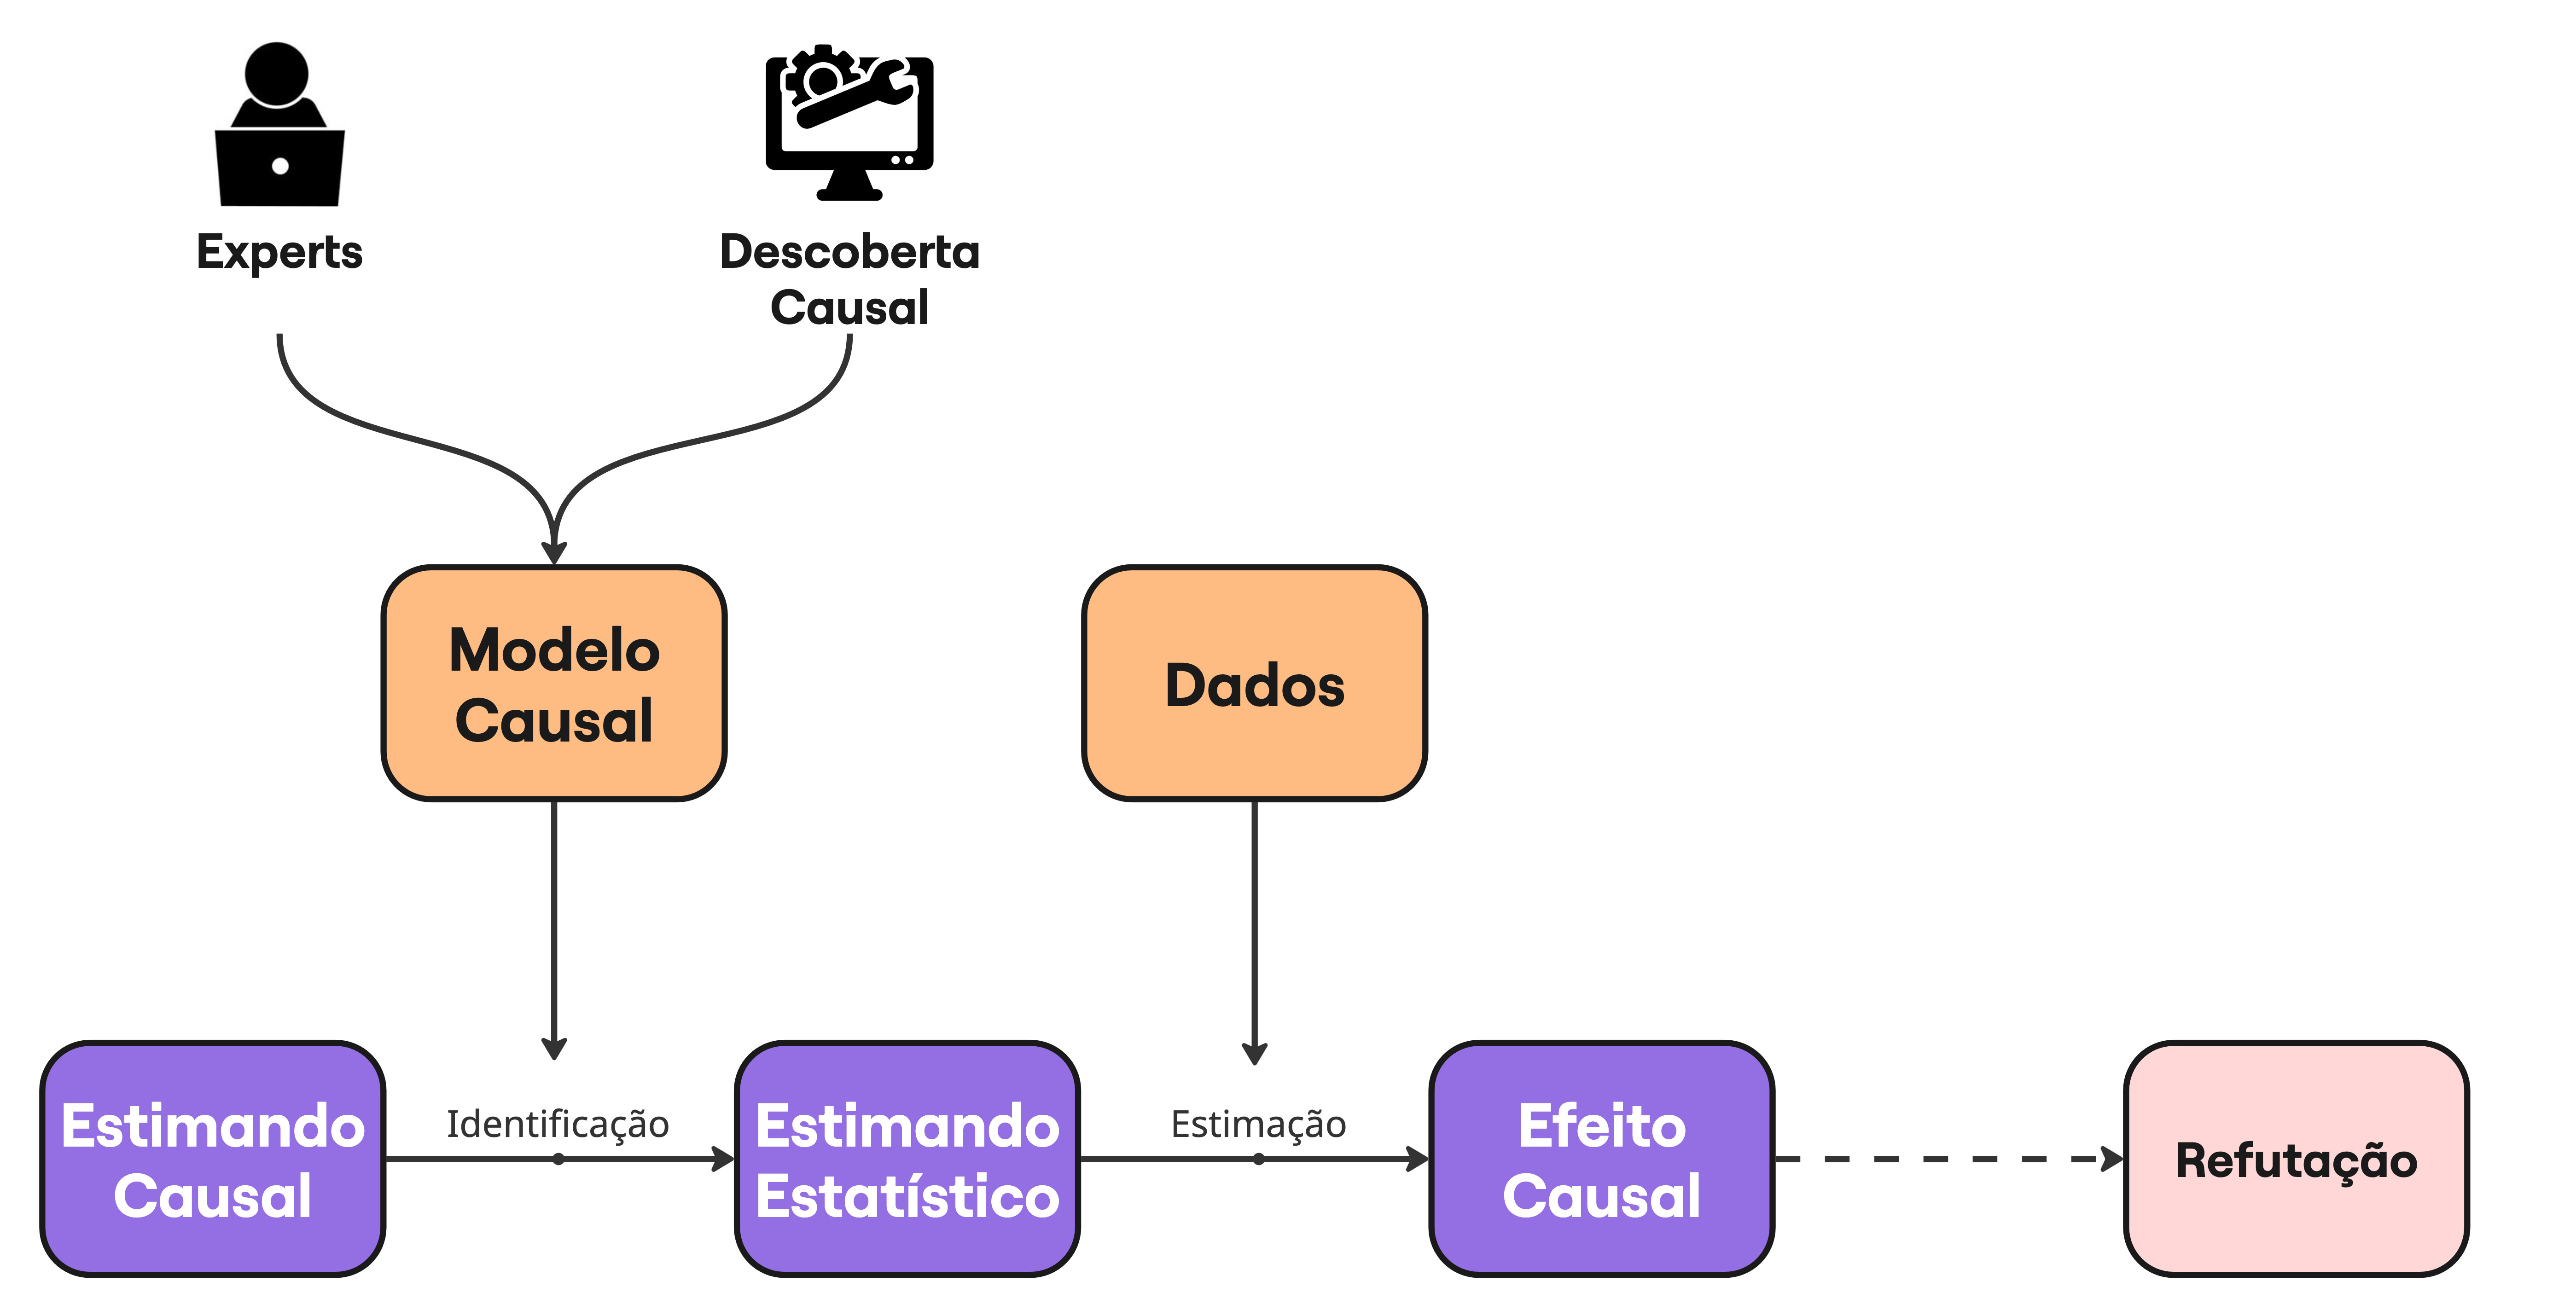
\includegraphics[width=1.0\framewidth]{figures/causal_inference_flow.jpg}
    \end{figure}
\end{frame}


\begin{frame}{Mão na massa}
	\notebooklink{3}{3\_causal\_estimation.ipynb}
\end{frame}

\begin{frame}[plain]{Inferência Causal}{E se o efeito não for igual pra todo mundo?}
    O ATE é uma média sobre toda a população. Só que médias escondem coisa.

    \pause
    Imagine um tratamento que ajuda metade das pessoas e atrapalha a outra metade, na mesma proporção. \pause O ATE dá quase zero \pause mas não porque o tratamento não faz nada, e sim porque os efeitos opostos se cancelam.

    \pause
    \vfill
    \begin{center}
        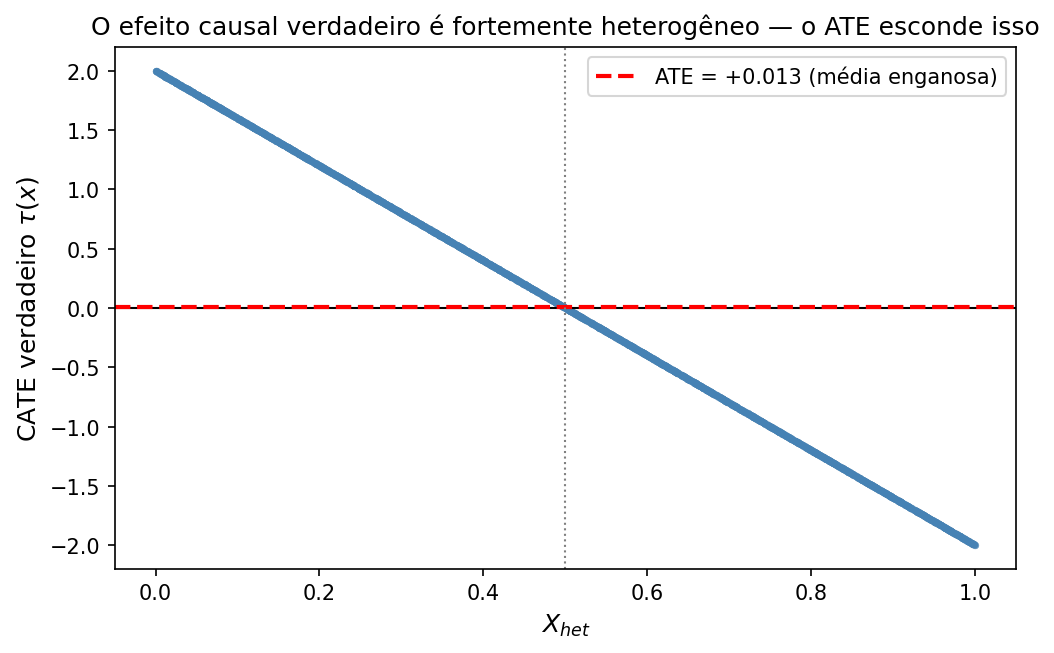
\includegraphics[width=0.625\linewidth]{figures/5_true_cate.png}
    \end{center}
\end{frame}

\begin{frame}{Inferência Causal}{CATE: o mesmo efeito, agora por subgrupo}
    O \textbf{CATE} (\textit{Conditional Average Treatment Effect}) responde: qual o efeito do tratamento, condicionado nas covariáveis \bm{$X$}?

    \vspace{10pt}
    \centering \bm{$\tau(x) = \mathbb{E}[Y(1) - Y(0) \mid X = x]$}
    \raggedright

    \pause
    \vspace{15pt}
    É a mesma ideia do ATE que você já viu, só que calculada separadamente pra cada perfil de unidade, em vez de uma média só pra todo mundo.

    \pause
    \vfill
    Com isso dá pra tomar uma decisão \textbf{personalizada}: trate a unidade \bm{$i$} só se \bm{$\hat\tau(x_i) > 0$}. Situações assim são comuns em saúde (um remédio ajuda um genótipo e prejudica outro) e marketing (uma promoção atrai quem é sensível a preço e irrita quem já é cliente fiel).
\end{frame}

\begin{frame}{Inferência Causal}{Meta-learners: estimando o CATE}
    A ideia por trás dos métodos mais comuns (\textit{meta-learners}) reaproveita os mesmos estimadores de ATE que você já viu, só que combinados de um jeito diferente:
    \begin{itemize}
        \item \textbf{S-learner}: um modelo só, com o tratamento como mais uma variável;
        \pause
        \item \textbf{T-learner}: dois modelos separados, um pra cada braço do tratamento;
        \pause
        \item \textbf{X-learner}: usa os dois modelos do T-learner pra imputar o efeito individual, útil quando os grupos são desbalanceados.
    \end{itemize}

    \begin{alertblock}{Notebook extra!}
		Caso queira aprofundar nesse assunto, veja o notebook extra \#5.
	\end{alertblock}
\end{frame}
